\documentclass[12pt]{comjnl}

\usepackage{amsmath}

%\copyrightyear{2009} \vol{00} \issue{0} \DOI{000}
\linespread{1.5}

\begin{document}

\title[Hashtag Segmentation of Conversational Tweets in Turkish]{Hashtag Segmentation of Conversational Tweets in Turkish, Modelling Segmentation Approach Midterm Report}
\author{Utku Saridede, Sevket Topuz}
\affiliation{Informational Retrival and Natural Language Processing, Department of
Computer Engineering, Bogazici University, Istanbul
Bebek 34342, TR} \email{utku.saridede@boun.edu.tr, sevket.topuz@boun.edu.tr}

\shortauthors{Saridede, Topuz}

\received{07 October 2016}
\revised{08 November 2016}

\keywords{Twitter; Tweets; Tweet; Hashtag; Segmentation; Turkish; Conversational Tweets;
		Hashtag Segmentation}

\begin{abstract}
Twitter is the latest social networking tool which affects everything related to the person.
Twitter allows its users to write at most 140 character long update, it is known off as 
``tweet''. In this research, analyzing segmentation of tweets is our main objective. There are
several researches in English, but not that much in Turkish. Studying with the Turkish corpus is
somehow hard to handle, because Turkish resources are insufficient. The usage of the hashtags
differ in country to country, that is, some countries do not know off proper usage of hashtags.
Having more than one word in the hashtag or lapsus calami are misusage, and prevent researhes 
to work properly. The other part of the project is analyzing hashtags in the way of linguistics.
Analyzed corpus will give more information about related countries. In the other words, short-term
hashtag analyses keep informed about spesific situations which influence the society.
\end{abstract}

\maketitle

\section{Introduction}
A hashtag is defined by any string prefixed with a ``\#'', for instance, “\#freedomtomark”,
“\#shesuggest”. The string can be a single word, an acronym, or multiple words joined
together, and usually identifies the subject topic of the tweet (e.g., “\#ENG493”)
or expresses a comment about it (e.g., “\#kappamevku”). 

The main objective is to implement machine learning based hashtag segmentation application.
Our first work was using twitter developer tools to 
extract tweets from their database. In the case of hashtag extraction, there are several issues. For instance,
we have recognized that Turkish people do not understand the usage of hashtag approach.
Therefore, the formation of corpus becomes difficult. Using large amount of raw data that 
is recieved from social media is the way of creating corpus. In the field of natural language 
processing, the main requirement is datasets. It clarifies why there is not enough
research in Turkish. Improving datasets might help researchers to test their idea and
modellings. 

The starting point of project is mainly based upon gathering data to avoid
backing to drawing point. That is, being blind to quantity of data causes to quit idea.
Existing methods of word segmentation unsuperwised language models. Researches claim that
using multiple corpora, the joint probability model from multiple corpora performs significantly 
better than the individual corpora. Weighted joint probability model, with weights is specific 
to each corpus. Decent approach is to train the weights in a supervised manner using max-margin 
methods, that is, a machine learning method to make a decision about the boundries of words.
The supervised probability models improve segmentation accuracy over joint probability models. 
Researchers observe that length of segments is an important parameter for word segmentation, and 
incorporating length-specific weights into our model supports the current model.
However the length specific models further improve segmentation accuracy over supervised 
probability models.

All mentioned models try to solve the problems with dynamic programming algorithms. The supervised length specific models have significantly more advencement over unsupervised single corpus and joint probability models. Segmentation of hashtags result in significant improvement in recall on searches for twitter trends.

\section{State of Art}

Word segmentation are of great interest to Natural Language Processing researchers. 
A good number of methods have been proposed in the literature, with quite good 
performances reported. There are several articles about word segmentation. 
There are two major categories, as well as, boundary prediction and word 
recognition. One of the most frequently used method
for that is maximum matching, by Wong and Chan – 1996. Many approaches help us to handle
unknown words and to get best proper answer in the case of ambiguity.

Boundary prediction methods usually utilize local statistics
to decide whether there is a word
boundary between two language units given the local context. The representative
examples involve Ando-Lee Criterion (Ando and Lee 2000),
Mutual Information (Sun, Shen, and Tsou 1998) and
Branching Entropy (Jin and Tanaka-Ishii 2006). Recently
Fleck (2008) proposed a algorithm called
WordEnds. It trained a boundary classifier with the dixit
boundary cues and then used it to mark word boundaries.
Zhikov, Takamura, and Okumura (2010) proposed
an efficient algorithm combining the strength of Minimum
Description Length approach and local statistics Branching Entropy.
High performance in terms of both accuracy and speed was
reported.

Word boundry detectiton
and word segmentation is very important for Chinese words research. A good survey about
Chinese word segmentation can be found out in Wu and Tseng's paper. A Chinese senteces do not
include delimiters to seperate words. It includes composed of a string of characters. Neural
networks and lazy learning approaches are methods that are used in word segmentation.

Another approach is word segmentation of URL links. To think about the word segmentation and
recognition problem for URL links, reasearchers adopt some basic principles from rule­based
approach. The dictionary should have sufficient amount of word entries. However, the occurence
of compound words makes it very difficult to match every component string exactly with the
dictionary entries. Evaluation of the hashtag segmentation has started to be improved with search engine
improvements of Twitter.

\section{Methods}
We have tried to discourse manly with 3 methods. Hashtag segmentation can be generally defined as word boundry detection. Because of this, we
start with detection of the word boundry. There are two feature­based learning methods,
Conditional Random Fields (CRFs)(Laerty et al.,2001) and Maximum Entropy (MaxEnt).
CRFs can represent the uncommon parts of the information as elements furthermore, are great at
displaying grouping marking problems. MaxEnt is extremely compelling at learning with a high
assortment of components, without agonizing over the multifaceted nature of the model. Hidden
Markov Model is a simplistic approach for word segmentation. It helps us to built character
trigrams. It tries to catch boundary characters that are current and previous ones. Peter Norvig's
implementation can be used for word bigrams.

Manual annotation is time consuming task and it limits the amount of trainig data that can be
created. We try to achieve utilizing data to create training sets for hashtag segmentation. Synthetic
hashtags by concatenating the words in tweets can also be used for training data because word
boundries are known. To use concatenating the words in tweets as training dataset, we need to filter
non­word tokens. If tweets include non­word token in the beginnig or end of the text, it can be
removed and other words can be used as trainig data. On the other side, if a non­word token appear
in the middle of the text, the tweet is dicarded because non­word token ib the middle of the tweet
may distort the word order. The word order is important point of trainig data.

We can use each character of training data to represent one function of learning system. Some
features should be determined and each character should be examined according to these features
to create machine learning system.

\section{Results}
The training data will be the part of the current data. We tokenize tweets, normalize them and get 
hashtags from them. 

\begin{figure}
\centering
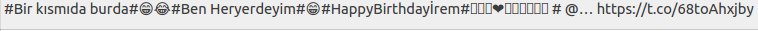
\includegraphics[width=3.5in]{tweet.png}
\caption{Tweet example.}\label{fig:Tweet}
\end{figure}

Implementing a method to get hashtags and insert them database is 
accomplished. There are two kind of table as well as "TEXTS" which contains unique tweet IDs
and tweet text. 

\begin{figure}
\centering
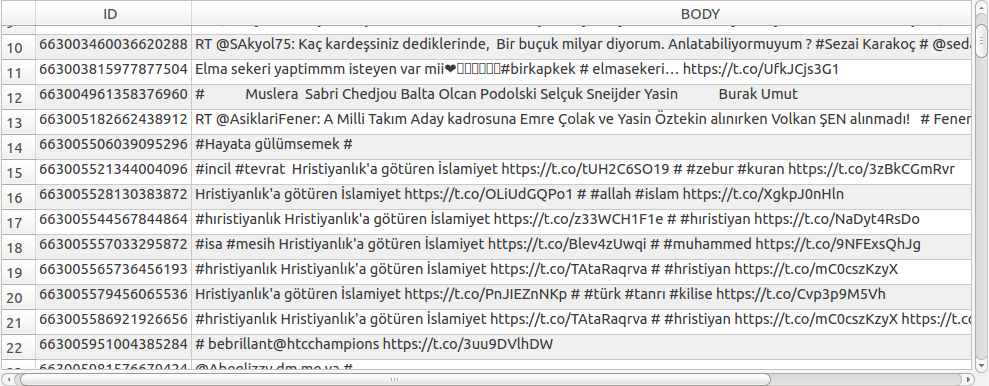
\includegraphics[width=3.5in]{text.png}
\caption{Text database table representation.}\label{fig:Tweet}
\end{figure}

The other one is "HASHTAGS" which contains tweet IDs and hashtags. Segmentation algorithm
is almost done.

\begin{figure}
\centering
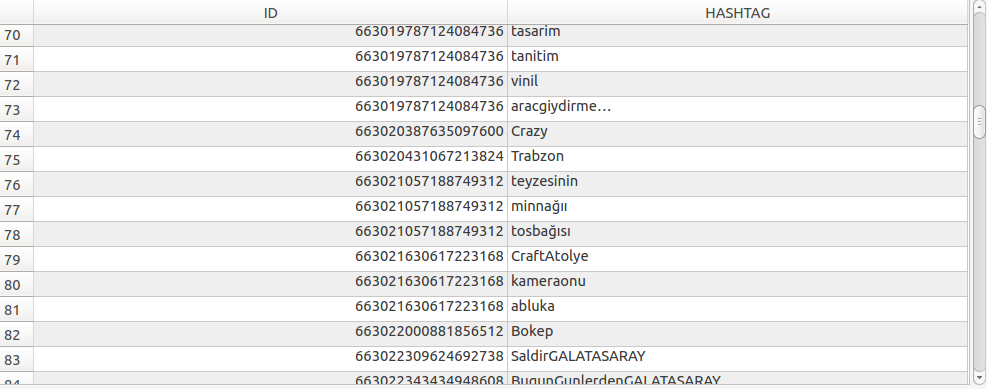
\includegraphics[width=3.5in]{hashtag.png}
\caption{Hashtag database table representation.}\label{fig:Hashtag}
\end{figure}

\section{Conclusion}
We proposed a simple and effective unsupervised
word segmentation approach. The criterion incorporates
boundary information to model words. 

\section{Future Work}
We decided to improve our segmentation algorithm. Features of the words will be dicussed. Training and real
datasets will be prepared. Every word in the training data will be used to improve machine
learning approach of our project. Later future works will be consulted with lecturer.

\section{References}
- Bansal, P., Bansal, R. and Varma V. 2015. Towards
Deep Semantic Analysis Of Hashtags. To Appear in
37th European Conference on Information Retrieval

- Berardi, G. and Esuli, A. and Marcheggiani, D. and
Sebastian, F. 2011. ISTI@TREC Microblog track
2011: exploring the use of hashtag segmentation
and text quality ranking.. In The Twentieth Text RE-
trieval Conference Proceedings

- Chen, S. and Xu Y. and Chang, H. 2012. A Sim-
ple and Effective Unsupervised Word Segmentation
Approach. Proceedings of the Twenty-Fifth AAAI
Conference on Artificial Intelligence

- Xue, N. 2003. Chinese word segmentation as charac-
ter tagging.. International Journal of Computational
Linguistics and Chinese Language Processing vol-
ume 8(1)

- Wong, P and Chan, C. 1996. Chinese word segmenta-
tion based on maximum matching and word binding
force. In the proceedings of the 16th conference on
Computational linguistics V(1) 200-203
\nocite{*}

\bibliographystyle{compj}
\bibliography{ModellingBidders}


\end{document}